\documentclass{article}
\usepackage{standalone}
\usepackage{mathrsfs}
\usepackage{tikz,interval}
\usetikzlibrary{matrix,arrows}
\begin{document}
\pagestyle{empty}

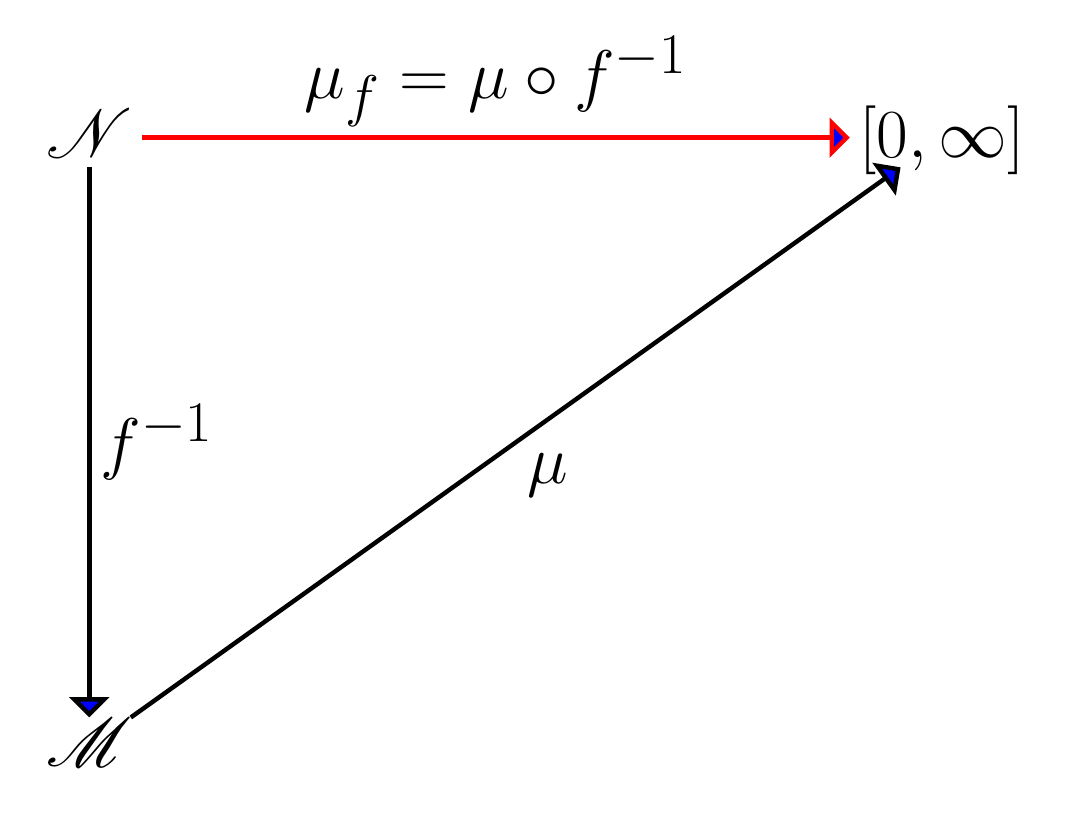
\begin{tikzpicture}[description/.style={fill=white,inner sep=2pt},font=\Huge]
    \matrix (m) [matrix of math nodes, row sep=3.5cm,
    column sep=4.5cm, text height=0.5cm, text depth=0.05ex]
    {\mathscr{N} & &\interval{0}{\infty} \\ 
	& & \\
	\mathscr{M} & &  \\};
    \path[draw=red,-triangle 90,fill=blue,ultra thick, font=\Huge] 
    (m-1-1) edge node[auto] {$\mu_{f} = \mu\circ f^{-1}$} (m-1-3);
    \path[draw=black,-triangle 90,fill=blue,ultra thick, font=\Huge] (m-1-1) edge node[auto] {$f^{-1}$}(m-3-1);
    \path[draw=black,-triangle 90,fill=blue,ultra thick, font=\Huge] (m-3-1) edge node[auto,swap] {$\mu$} (m-1-3);
\end{tikzpicture}
\end{document}
